\documentclass{article}
\usepackage{amsmath}
\usepackage{graphicx}
\usepackage{url}
\graphicspath{{images/}}

% Margins
\topmargin=-0.45in
\evensidemargin=0in
\oddsidemargin=0in
\textwidth=6.5in
\textheight=9.0in
\headsep=0.25in

%Title Info
\title{\vspace{-2cm}Particle Filters} %remove the extra spacing at the top
\author{Alex Pan and Alec Kosik}
\date{} %blank the date

\begin{document}
\maketitle

% --------------------- Abstract ---------------------
\begin{abstract}
Particle Filters allow us to model non-linear and non-Gaussian distributions through Monte Carlo methods. We first discuss HMM, and then discuss a recursive formulation of the distribution of $p(x_t|y_{1:n})$. We then discuss how this leads well to an algorithmic approach. Finally, we investigate Kalman Filters, Importance Sampling, and SIR. We discuss the motivations for and relevant problems with each approach.
\end{abstract}

\section{Introduction}

% --------------------- Preliminaries ---------------------
\section{Hidden Markov Models}

A \textbf{Hidden Markov Model} (HMM) is defined as a Markov process with states that cannot be observed, but gives outputs that are dependent on the hidden state of the system. If we let the random variable $X_i$ represent the $i$-th state of the system, and the random variable $Y_i$ represent the $i$-th output of the system, we have:
\begin{equation}
X_1 \sim \mu (x_1) \textnormal{ and } X_n|(X_{n-1}=x_{n-1}) \sim f(x_n|x_{n-1})
\end{equation}
\begin{equation}
Y_n|(X_n = x_n) \sim g(y_n|x_n)
\end{equation}
where $X_1$ is defined by some initial conditions $\mu(x_1)$. Note how $f$ obeys the Markov property, so the current state $x_n$ is dependent only on the previous state $x_{n-1}$. Also note that $g$ shows that the current observation $y_n$ is only dependent on the current state $x_n$.

Let $x_{1:n}$ represent the ordered n-tuple of hidden states $(x_1,\dots,x_n)$ where $x_i$ is the $i$-th hidden state. Similarly, let $y_{1:n}$ represent the ordered n-tuple of observations $(y_1,\dots,y_n)$. There are a few important distributions that follow directly from our HMM setting.
% this derivation is confusing (1) because of the switch from p to f and (2) because of the application of bayes rule to get derive line 2. i think it would be better to just give the equation in 1 line and explain where it comes from in prose.
\begin{equation} \label{p(x_{1:n})}
\begin{split}
p(x_{1:n})
&= p(x_1)p(x_2|x_1)p(x_3|x_2,x_1)\dots p(x_n|x_{n-1},\dots,x_1)\\
&= p(x_1)p(x_2|x_1)p(x_3|x_2)\dots p(x_n|x_{n-1})\\
&=\mu(x_1)\prod_{i=2}^{n} f(x_i|x_{i-1})\\
\end{split}
\end{equation}

\begin{equation} \label{p(y_{1:n}|x_{1:n})}
\begin{split}
p(y_{1:n}|x_{1:n})
&= p(y_1|x_{1:n})p(y_2|x_{1:n},y_1)(y_3|x_{1:n},y_2,y_1)\dots (y_n|x_{1:n},y_{n-1},\dots,y_1)\\
&= p(y_1|x_1)p(y_2|x_2)\dots (y_n|x_n)\\
&= \prod_{i=1}^{n} g(y_i|x_i)\\
\end{split}
\end{equation}


% --------------------- Setting up the problem ---------------------
\section{Particle Filters}
\subsection{General Goals}
There are a few different uses of the particle filtering method. We could model the distribution $p(x_{1:n}|y_{1:n})$, the distribution $p(x_n|y_{1:n})$, or even the expected value of functions defined on these distributions. Here, our main goal is to use our observations to determine the hidden state of the system. That is, we want to figure out $p(x_{n}|y_{1:n})$. Recognizing that this is a marginal is useful because then we can just say:

\begin{equation}
p(x_{n}|y_{1:n}) = \int p(x_{1:n}|y_{1:n}) dx_{1:n-1}
\end{equation}

Setting our goal as a marginal of $p(x_{1:n}|y_{1:n})$ is helpful because we can refactor the full conditional distribution to see how it comes from our prior distributions derived in \eqref{p(x_{1:n})} and \eqref{p(y_{1:n}|x_{1:n})}. Refactoring and using our initial HMM conditions, we can show:

\begin{equation}
\begin{split}
p(x_{1:n}|y_{1:n}) &= \frac{p(x_{1:n},y_{1:n})}{p(y_{1:n})}\\
&= \frac{p(x_{1:n}) p(y_{1:n}|x_{1:n})}{p(y_{1:n})}\\
&= \frac{p(x_{1:n}) p(y_{1:n}|x_{1:n})}{\int p(x_{1:n},y_{1:n}) dx_{1:n}}\\
&= \frac{\mu(x_1)\prod_{i=2}^{n} f(x_1|x_{i-1})\prod_{i=1}^{n} g(y_i|x_i)}{\int \mu(x_1)\prod_{i=2}^{n} f(x_1|x_{i-1})\prod_{i=1}^{n} g(y_i|x_i) dx_{1:n}}
\end{split}
\end{equation}

Thus,

\begin{equation}
p(x_n|y_{1:n}) = \int \frac{\mu(x_1)\prod_{i=2}^{n} f(x_1|x_{i-1})\prod_{i=1}^{n} g(y_i|x_i)}{\int \mu(x_1)\prod_{i=2}^{n} f(x_1|x_{i-1})\prod_{i=1}^{n} g(y_i|x_i) dx_{1:n}} dx_{1:n-1}
\end{equation}

This looks really messy, but it's helpful to see that this is just integration of functions we already know: $f$ and $g$. In other words, we already have all the information we need to arrive at the answer.

\subsection{A Recursive Formulation}
% not integrable, we can't calculate this equation. also, i don't think it's closed-form or analytical since it contains an integral. there must be some word for it.
While we now have a nice equation, it would be really inefficient if we had to calculate this whole equation every single iteration of our system. Instead, we can formulate this recursively and see how some of the values carry through. This recursiveness is described in two parts: the update equation and the prediction equation. We show the update equation first:

\begin{equation} \label{want}
p(x_t|y_{0:t}) = \frac{p(x_t|y_{0:t-1})p(y_t|x_t)}{p(y_t|y_{0:t-1})}
\end{equation}

The derivation will be broken into 2 parts. First, we will show that \eqref{want} holds iff $p(x_t,y_{0:t}) = p(x_t,y_{0:t-1})p(y_t|x_t)$ holds. Then we will show that $p(x_t,y_{0:t}) = p(x_t,y_{0:t-1})p(y_t|x_t)$. We start by applying Bayes' rule to the left side of \eqref{want} and then moving the denominator to the right side:

\begin{align*}
p(x_t,y_{0:t}) &= \frac{p(x_t|y_{0:t})p(y_t|x_t)}{p(y_t|y_{0:t-1})}p(y_{0:t}) \\
\intertext{Applying Bayes' rule to $p(x_t|y_{0:t})$:}
&= \frac{p(x_t,y_{0:t})p(y_t|x_t)}{p(y_t|y_{0:t-1})p(y_{0:t-1})}p(y_{0:t}) \\
&= \frac{p(x_t,y_{0:t})p(y_t|x_t)}{p(y_{0:t})}p(y_{0:t}) \\
&= p(x_t,y_{0:t})p(y_t|x_t)
\end{align*}

\noindent
Second, we show $p(x_t,y_{0:t}) = p(x_t,y_{0:t-1})p(y_t|x_t)$. Let's start by refactoring the right-side.
\begin{align*}
p(x_t,y_{0:t-1})p(y_t|x_t) &= p(x_t|y_{0:t-1})p(y_{0:t-1})\frac{p(x_t,y_t)}{p(x_t)}\\
&= p(x_t|y_{0:t-1})p(y_{0:t-1})\frac{p(x_t|y_t)p(y_t)}{p(x_t)}\\
\intertext{Using the fact that: $p(x|yz) =$ {\Large $\frac{p(y)p(z)}{p(yz)}\frac{p(x|y)p(x|z)}{p(x)}$}
  Let: $x=x_t, y=y_{0:t-1}, z = y_t,$}
\intertext{We can now see that:  $p(x_t|y_{0:t-1},y_t) =$ {\Large $\frac{p(y_{0:t-1})p(y_t)}{p(y_{0:t-1},y_t)}\frac{p(x_t|y_{0:t-1})p(x_t|y_t)}{p(x_t)}$}}
\intertext{Thus,}
p(x_t|y_{0:t-1})p(y_{0:t-1})\frac{p(x_t|y_t)p(y_t)}{p(x_t)} &= p(x_t|y_{0:t})p(y_{0:t})\\
&= p(x_t,y_{0:t})\\
\end{align*}

\noindent
We now show how to derive the prediction equation:
\begin{equation}
p(x_t|y_{0:t-1}) = \int f(x_t|x_{t-1})p(x_{t-1}|y_{0:t-1}) dx_{t-1}
\end{equation}

\noindent
If we approach this as a marginal by integrating out $x_{t-1}$ we normally would formulate this as:

\begin{equation}
\begin{split}
p(x_t|y_{0:t-1}) &= \int p(x_{t-1:t}|y_{0:t-1}) dx_{t-1}\\
&= \int p(x_t|x_{t-1},y_{0:t-1})p(x_{t-1}|y_{0:t-1}) dx_{t-1}\\
\end{split}
\end{equation}
We can make use of the Markov property to see:
\begin{equation}
p(x_t|x_{t-1},y_{0:t-1}) = p(x_t|x_{t-1}) = f(x_t|x_{t-1})
\end{equation}



--------Some more words explaining what exactly just happened should go here.----------

The issue now is that this is sometimes intractable. If functions are nice, like guassians or linear distributions, this is integrable and we can arrive at a solution analytically. However, this is not always the case, which is why we sometimes need to derive an answer from numeric approximations.

% --------------------- Kalman Filter ---------------------
\section{Kalman Filter}

This needs to be re-done because I've moved the discussion of the recursive form to the earlier section. Former code has been commented out.
% So let's say you're really lucky and your initial distribution is something nice. This allows us to get a solution analytically through a method called the Kalman Filter. The algorithm becomes a little more obvious if we recognize the recursive form of our goal:

% \begin{equation}
% \textnormal{Prediction step:  }
% p(x_{n}|y_{1:n-1}) = \int f(x_n|x_{n-1})p(x_{n-1}|y_{1:n-1}) dx_{n-1}
% \end{equation}

% \begin{equation}
% \textnormal{Update step:  }
% p(x_{n}|y_{1:n}) = \frac{g(y_n|x_n)p(x_{n}|y_{1:n-1})}{p(y_n|y_{1:n-1})}
% \end{equation}

% Essentially, we are now assuming that $p(x_{n-1}|y_{1:n-1})$ is known due to recursion. To see how this relates to our earlier definition of $p(x_{n}|y_{1:n})$ in Eq. (4), note that the numerator of Eq. (4) is the product of all of $f$ and $g$ from Eq. (5) and (6) while the denominator is the product of conditionals from Eq. (6). The denominator simplifies to $p(y_{1:n})$ which is just the marginal distribution of observations on the joint, hence the second integral inside of the denominator of Eq. (4).

% --------------------- SMC Methods ---------------------
\section{Sequential Monte Carlo Methods}

So what if our distribution isn't nice? We will use Monte Carlo Methods to approximate Eq. (5) and (6):

\begin{equation}
\textnormal{Prediction step:  }
\pi_{x_{1:t}|y_{1:t-1}}(x_{1:t}|y_{1:t-1})= f(x_t|x_{t-1}) \pi_{x_{1:t-1}|y_{1:t-1}}(x_{1:t-1}|y_{1:t-1})
\end{equation}

\begin{equation}
\textnormal{Update step:  }
\pi_{x_{1:t}|y_{1:t}}(x_{1:t}|y_{1:t})\propto g(y_t|x_t)\pi_{x_{1:t}|y_{1:t-1}}(x_{1:t}|y_{1:t-1})
\end{equation}

% --------------------- SIS ---------------------
\section{SIS}

\begin{enumerate}
\item \textit{Initialization:}
\item[] For $i=1,\dots N$:
\begin{itemize}
\item[] Sample $x_0^{(i)} \sim \mu(x_0)$
\item[] Assign weights $\widetilde{w}_0^{(i)} = g(y_0|x_0^{(i)})$
\item[] Normalize weights $w_0^{(i)} = \frac{\widetilde{w}_0^{(i)}}{\sum_{i=1}^{n} \widetilde{w}_0^{(i)}}$
\end{itemize}
\item \textit{Importance Sampling:}
\item[] For $t=1,\dots,T$:
\begin{itemize}
\item[] Sample $x_t^{(i)} \sim f(x_t|x_{t-1}^{i})$
\item[] Assign weights $\widetilde{w}_t^{(i)} = g(y_t|x_t^{(i)})$
\item[] Normalize weights $w_t^{(i)} = \frac{\widetilde{w}_t^{(i)}}{\sum_{i=1}^{n} \widetilde{w}_t^{(i)}}$
\end{itemize}
\item Return $\{x_T^{(i)},w_T^{(i)}\}_{i=1}^N$
\end{enumerate}

To algorithmically find our target distribution, we sample from something simple like the Uniform or Gaussian distribution. We then weight these samples using our observations and $g$. Essentially, we iterate between (7) and (8), sampling new points and updating our weights each time. While this sounds okay, it turns out that we never use SIS in real life because of something called the ``degeneracy problem''.

% --------------------- Degeneracy Problem ---------------------
\section{Degeneracy Problem}
When we are sampling from our reweighted distribution, it is possible that certain points are assigned very low weight. In future iterations, this is likely to compound, making their weights essentially negligible. This manifests as a handful of points having nearly all the weight while the rest of our points have ``degenerated''. This is a problem because our distribution essentially is now defined by just a few of the original points we started with, which is not enough to get an accurate representation of our target distribution.


% --------------------- Bootstrap/SIR ---------------------
\section{Bootstrap (SIR)}
We can effectively solve the degeneracy problem by resampling. After each iteration $t>0$ we will resample all $N$ particles from the weighted distribution defined in the previous time step. Thus particles with low-to-negligible weights at $t$ will have a low probability of persisting to $t+1$. See Figure \ref{fig:sir} for a visualization of this process.

\begin{enumerate}
\item \textit{Initialization:}
\item[] For $i=1,\dots N$:
\begin{itemize}
\item[] Sample $x_0^{(i)} \sim \mu(x_0)$
\item[] Assign weights $\widetilde{w}_0^{(i)} = g(y_0|x_0^{(i)})$
\item[] Normalize weights $w_0^{(i)} = \frac{\widetilde{w}_0^{(i)}}{\sum_{i=1}^{n} \widetilde{w}_0^{(i)}}$
\end{itemize}
\item \textit{Importance Sampling:}
\item[] For $t=1,\dots,T$:
\begin{itemize}
\item[] Sample $x_t^{(i)} \sim f(x_t|\widetilde{x}_{t-1}^{i})$
\item[] Assign weights $\widetilde{w}_t^{(i)} = g(y_t|x_t^{(i)})$
\item[] Normalize weights $w_t^{(i)} = \frac{\widetilde{w}_t^{(i)}}{\sum_{i=1}^{n} \widetilde{w}_t^{(i)}}$
\item[] Resample $\widetilde{x}_t^{(i)}$ from $x_t^{(i)}$ according to the weight distribution with replacement.
\end{itemize}
\item Return $\{x_T^{(i)},w_T^{(i)}\}_{i=1}^N$
\end{enumerate}

\begin{figure}
\centering
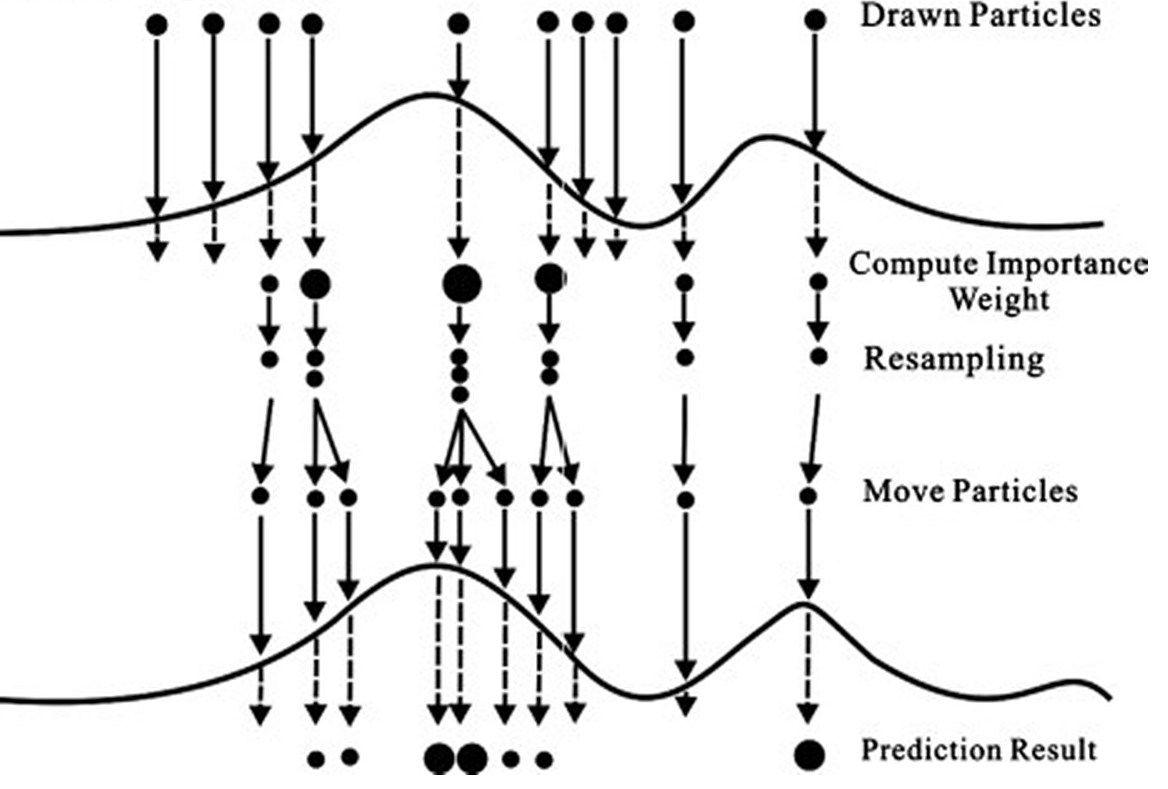
\includegraphics[scale=.25]{sir}
\caption{The SIR algorithm, adopted from \cite{sirfig}.}
\label{fig:sir}
\end{figure}

While this addresses the degeneracy problem, it turns out that resampling has it's own issue which we call the ``sampling impoverishment problem''. This comes about because our higher weighted points are more likely to be drawn multiple times. Instead of having many low-weight points spread out across the state-space---in the case of SIS and the degeneracy problem---we will have lots of evenly-weighted points concentrated around areas where high-weight points originally occurred. Intuitively, the degeneracy problem leaves you with a diverse scattering of point masses with a few ill-defined peaks while the sampling impoverishment problem leaves you with \textit{only} well defined peaks. There are methods that address both of these issues but they require fancy sounding things like the ``Epanechnikov Kernel'', which our outside the scope of our discussion. It turns out that SIR is generally good enough and is the algorithm that people generally use.

\section{Conclusion}



% --------------------- Some equations!!! ---------------------

% \section{Lots of equations we'll use:}
% \begin{equation}
% \textnormal{Prior: }
% p(x_{1:n}) = \mu(x_1)\prod_{i=2}^{n} f(x_1|x_{i-1})
% \end{equation}

% \begin{equation}
% \textnormal{Conditional of Y: }
% p(y_{1:n}|x_{1:n}) = \prod_{i=1}^{n} g(y_i|x_i)
% \end{equation}

% \begin{equation}
% \textnormal{Conditional of X: }
% p(x_{1:n}|y_{1:n}) = \frac{p(x_{1:n},y_{1:n})}{p(y_{1:n})}
% \end{equation}

% \begin{equation}
% \textnormal{Joint: }
% p(x_{1:n},y_{1:n}) = p(x_{1:n}) p(y_{1:n}|x_{1:n})
% \end{equation}

% \begin{equation}
% \textnormal{Marginal: }
% p(y_{1:n}) = \int p(x_{1:n},y_{1:n}) dx_{1:n}
% \end{equation}

% \begin{equation}
% \textnormal{We have: }
% \{p(x_{1:n}|y_{1:n})\}_{n>0}
% \textnormal{ and }
% \{p(y_{1:n})\}_{n>0}
% \end{equation}

% \begin{equation}
% \textnormal{Want to find: }
% \{p(x_n|y_{1:n})\}_{n>0}
% \end{equation}

% \begin{equation}
% \textnormal{Reformulate the joint: }
% p(x_{1:n},y_{1:n}) = p(x_{1:n-1},y_{1:n-1}) f(x_n|x_{n-1}) g(y_n|x_n)
% \end{equation}

% \begin{equation}
% \begin{split}
% p(x_{1:n},y_{1:n}) &= p(x_{1:n}) p(y_{1:n}|x_{1:n})\\
% p(x_{1:n}) &= \mu(x_1)\prod_{i=2}^{n} f(x_1|x_{i-1})
% = (\mu(x_1)\prod_{i=2}^{n-1} f(x_1|x_{i-1})) f(x_n|x_{n-1})
% = p(x_{1:n-1} (x_n|x_{n-1}))\\
% p(y_{1:n}|x_{1:n}) &= \prod_{i=1}^{n} g(y_i|x_i)
% = (\prod_{i=1}^{n-1} g(y_i|x_i)) g(y_n|x_n)
% = p(y_{1:n-1}|x_{1:n-1}) g(y_n|x_n)\\
% p(y_{1:n-1}|x_{1:n-1}) &= \frac{p(x_{1:n-1},y_{1:n-1})}{p(y_{1:n-1})}\\
% p(x_{1:n},y_{1:n}) &= p(x_{1:n-1} (x_n|x_{n-1})) \frac{p(x_{1:n-1},y_{1:n-1})}{p(y_{1:n-1})} g(y_n|x_n)
% = p(x_{1:n-1},y_{1:n-1}) f(x_n|x_{n-1}) g(y_n|x_n)
% \end{split}
% \end{equation}

% \begin{equation}
% \textnormal{Reformulate the conditional of X: }
% p(x_{1:n}|y_{1:n}) = p(x_{1:n-1}|y_{1:n-1})\frac{f(x_n|x_{n-1}) g(y_n|x_n)}{p(y_n|y_{1:n-1})}
% \end{equation}

% \begin{equation}
% \begin{split}
% p(x_{1:n}|y_{1:n}) &= \frac{p(x_{1:n},y_{1:n})}{p(y_{1:n})}\\
% p(x_{1:n},y_{1:n}) &= p(x_{1:n-1},y_{1:n-1}) f(x_n|x_{n-1}) g(y_n|x_n)\\
% p(x_{1:n-1},y_{1:n-1}) &= p(y_{1:n-1}) p(x_{1:n-1}|y_{1:n-1})\\
% p(y_{1:n-1}) &= \frac{p(y_{1:n-1},y_n)}{p(y_n|y_{1:n-1})} = \frac{p(y_{1:n})}{p(y_n|y_{1:n-1})}\\
% p(x_{1:n}|y_{1:n}) &= \frac{1}{p(y_{1:n})}\frac{p(y_{1:n})}{p(y_n|y_{1:n-1})} p(x_{1:n-1}|y_{1:n-1}) f(x_n|x_{n-1}) g(y_n|x_n)\\
% &= p(x_{1:n-1}|y_{1:n-1})\frac{f(x_n|x_{n-1}) g(y_n|x_n)}{p(y_n|y_{1:n-1})}\\
% \end{split}
% \end{equation}

% \begin{equation}
% \pi_n(x_{1:n})=p(x_{1:n}|y_{1:n}) = \frac{p(x_{1:n},y_{1:n})}{p(y_{1:n})}
% \end{equation}

% \begin{equation}
% \hat{\pi}_n(x_{1:n})=\frac{1}{N}\sum_{i=1}^{N}\delta_{X_{1:n}^i}(x_{1:n})
% \end{equation}

% \begin{equation}
% \hat{\pi}_n(x_k)=\frac{1}{N}\sum_{i=1}^{N}\delta_{X_k^i}(x_k)
% \end{equation}

\newpage
\bibliography{Reportbib}
\bibliographystyle{ieeetr}

\end{document}
